\documentclass[mat1]{fmfdelo}
% \documentclass[fin1]{fmfdelo}
% \documentclass[isrm1]{fmfdelo}
% \documentclass[mat2]{fmfdelo}
% \documentclass[fin2]{fmfdelo}
% \documentclass[isrm2]{fmfdelo}

% naslednje ukaze ustrezno napolnite
\avtor{Izak Jenko}

\naslov{Kompleksni torusi in eliptične krivulje}
\title{Complex tori and elliptic curves}

% navedite ime mentorja s polnim nazivom: doc.~dr.~Ime Priimek,
% izr.~prof.~dr.~Ime Priimek, prof.~dr.~Ime Priimek
% uporabite le tisti ukaz/ukaze, ki je/so za vas ustrezni
\mentor{izr.~prof.~dr.~Sašo Strle}
% \mentorica{}
% \somentor{}
% \somentorica{}
% \mentorja{}{}
% \mentorici{}{}

\letnica{2021} % leto diplome

%  V povzetku na kratko opišite vsebinske rezultate dela. Sem ne sodi razlaga organizacije dela --
%  v katerem poglavju/razdelku je kaj, pač pa le opis vsebine.
\povzetek{}

%  Prevod slovenskega povzetka v angleščino.
\abstract{}

% navedite vsaj eno klasifikacijsko oznako --
% dostopne so na www.ams.org/mathscinet/msc/msc2020.html
\klasifikacija{}
\kljucnebesede{} % navedite nekaj ključnih pojmov, ki nastopajo v delu
\keywords{} % angleški prevod ključnih besed

\zapisiMetaPodatke  % poskrbi za metapodatke in veljaven PDF/A-1b standard

% aktivirajte pakete, ki jih potrebujete
% \usepackage{tikz}
\usepackage{bm}
\usepackage[dvipsnames]{xcolor}
\usepackage{array}
\usepackage{faktor}
\usepackage{caption}
\usepackage{xfrac}
\usepackage[shortlabels]{enumitem}
% \usepackage{physics}

%%%

\usepackage{amsmath}
\usepackage{array}
\usepackage{tikz}
\usetikzlibrary{decorations.pathreplacing}
\newcommand{\tikzmark}[1]{\tikz[overlay,remember picture,baseline=(#1.base)]
  \node (#1) {\strut};}

%%%  

\newcommand{\R}{\mathbb R}
\newcommand{\N}{\mathbb N}
\newcommand{\Z}{\mathbb Z}
\newcommand{\C}{\mathbb C}
\newcommand{\CM}{\mathbb C ^\times}
\newcommand{\PC}{P^2(\mathbb C)}
\newcommand{\Q}{\mathbb Q}
\newcommand{\RS}{\widehat{\C}}
\newcommand{\Cxyz}{\C[x,y,z]}
\newcommand{\linphi}{\mathcal{A}_\Phi}
\newcommand{\oio}{\pcoor{0: 1 : 0}}
\newcommand{\om}{\omega}
\newcommand{\inv}{^{-1}}
\newcommand{\torus}{\C/\Lambda}
\newcommand{\elf}{\C(\Lambda)}

\newcommand{\pcoor}[1]{%
  \begingroup\lccode`~=`: \lowercase{\endgroup
  \edef~}{\mathbin{\mathchar\the\mathcode`:}\nobreak}%
  [% opening symbol
  \begingroup
  \mathcode`:=\string"8000
  #1%
  \endgroup
  ]% closing symbol
}

\newcommand{\pdv}[2][]{\frac{\partial#1}{\partial#2}}

\newcommand{\bigslant}[2]{{\raisebox{.2em}{$#1$}\left/\raisebox{-.2em}{$#2$}\right.}}

% \newcommand{\res}[2]{\operatorname{res}_{#1}\left(#2\right)}
% \newcommand{\ord}[2]{\operatorname{ord}_{#1}\left(#2\right)}

\newcommand{\res}[2]{\operatorname{res}_{#1}(#2)}
\newcommand{\ord}[2]{\operatorname{ord}_{#1}(#2)}

\newcommand{\hol}[1]{\mathcal{O}(#1)}

\newcommand{\abs}[1]{\left\lvert #1 \right\rvert}

\newcommand{\disk}[2]{\Delta(#1, #2)}

%command for alg-closure that automatically adapts its 'bar' to the arg based on the args length (including '\')
\newcommand{\ols}[1]{\mskip.5\thinmuskip\overline{\mskip-.5\thinmuskip {#1} \mskip-.5\thinmuskip}\mskip.5\thinmuskip} % overline short
\newcommand{\olsi}[1]{\,\overline{\!{#1}}} % overline short italic


\newcommand{\kom}[1]{
    \textcolor{RoyalBlue}{//#1}
}


% matematične operatorje deklarirajte kot take, da jih bo Latex pravilno stavil
% \DeclareMathOperator{\conv}{conv}

\DeclareMathOperator{\GL}{GL}
\DeclareMathOperator{\Aut}{Aut}
\DeclareMathOperator{\rang}{rang}
\DeclareMathOperator{\id}{id}

% vstavite svoje definicije ...
%  \newcommand{}{}

\theoremstyle{definition}
\newenvironment{komentar}[1][Komentar]{\begin{proof}[#1]\let\qed\relax}{\end{proof}}

\begin{document}

%--------------------------------------------------------------------------%
%%%%%%%%%%%%%%%%%%%%%%%%%%%%%% 1. UVOD %%%%%%%%%%%%%%%%%%%%%%%%%%%%%%%%%%%%%
%--------------------------------------------------------------------------%

\section{Uvod}

Matematike pogosto zanimajo rešitve različnih enačb. Obstoj rešitev, kakšne lastnosti imajo in
kako se obnašajo pod raznimi transformacijami. Osrednja tema moje naloge bo preučiti in ustvariti
geometrijsko predstavo množice ničel kompleksnega polinoma tretje stopnje posebne oblike. 
To množico ničel si lahko predstavljamo kot realno ploskev in ji pravimo eliptična krivulja.   
Zgodovinsko je eliptična krivulja množica ničel enačbe
\[
    y^2 = x^3 + ax + b. 
\]
V tem delu pa se bomo ukvarjali z nekoliko prilagojeno -- projektivno -- obliko te enačbe. Množicam ničel
polinomov več spremenljivk pravimo \emph{algebraične krivulje} in z njimi bomo začeli v poglavju \ref{algebraicne krivulje}. 
\par 
Pri iskanju rešitev
polinomskih enačb se razmeroma hitro porodi vprašanje, iz katerega ambientnega prostora 
sploh sprejemamo veljavne rešitve. Spomnimo se fundametalnega izreka algebre, ki pravi, da ima
vsak nekonstanten polinom s kompleksnimi koeficienti ničlo v polju kompleksnih števil, med tem
ko brez težav poiščemo realne polinome, ki realnih ničel nimajo. Podobno situacijo imamo tukaj. 
Eliptične krivulje se namreč da študirati nad mnogo različnimi polji. Nad končnimi polji igrajo
eliptične kriulje pomembno vlogo v kriprografiji, nad racionalnimi števili v algebraični teoriji
števil, mi pa jih bomo v tem delu gledali nad poljem kompleksnih števil. 
\par
V primeru obravnave nad poljem kompleksnih števil eliptične
krivulje naravno pridobijo dodatno kompleksno stukturo in na ta način postanejo t.~i.\ \emph{Riemannove ploskve}. Ta struktura nam omogoča analizo holomorfnih funkcij na prostorih, ki niso nujno domene v kompleksni ravnini in jo
bomo bolj podrobno preiskali v poglavju \ref{riemannove ploskve}. V nadaljevanju bomo videli, da tudi torus premore strukturo Riemannove ploskve in ga bomo skupaj s to strukturo imenovali kompleksni torus. Izkaže se, da je kompleksni
torus najbolj smiselna domena dvojno periodičnih oz. eliptičnih funkcij. Lastnosti in obnašanje eliptičnih funkcij si bomo ogledali v poglavju \ref{elipticne funkcije}, klučno vlogo pa bo igrala prav posebna Weierstrassova eliptična funkcija $\wp$. Ta nam bo nazadnje v poglavju \ref{poglavje izomorfizem} omogočila konstrukcijo preslikave, ki bo pokazala, da sta kompleksni torus in eliptična krivulja v nekem smislu enaka matematična objekta.

Vredno je še opomniti, da eliptične krivulje in področja, v katerih se uporabljajo,
nimajo več vsebinsko praktično nič opravka z elipsami. 
Izkazalo se je, da so inverzi funkcij, s katermi računamo dolžine lokov elips, dvojno periodični oz. eliptični,
če jih gledamo kot funkcije kompleksne spremenljivke. Te dvojno periodične funkcije pa so tesno povezane z enačbo,
ki ji zadoščajo eliptične krivulje in se bomo k njim vrnili v poglavju \ref{elipticne funkcije}.

%--------------------------------------------------------------------------%
%%%%%%%%%%%%%%%%%%%%%% 2. ALGEBRAIČNE KRIVULJE %%%%%%%%%%%%%%%%%%%%%%%%%%%%%
%--------------------------------------------------------------------------%

\section{Algebraične krivulje} \label{algebraicne krivulje}
Algebraične krivulje so množice ničel polinomov nad različnimi polji. V tem poglavju bomo začeli 
z afinimi
algebraičnimi krivuljami, ki jih v nadaljevanju sicer ne bomo direktno potrebovali, bodo pa igrale pomembno
vlogo pri razumevanju projektivnih algebraičnih krivulj, ki jih bomo vpeljali takoj za tem. 
Zaradi namenov tega dela, algebraičnih krivulj ne bomo obravnavali nad povsem splošnimi polji, pač pa se
bomo omejili na polje kompleksnih števil, ki ga bomo označevali s $\C$. V smislu enodimenzionalnega kompleksnega prostora bomo množici kompleksnih števil pravili tudi kompleksna premica.

%%%%% Afine algebraične krivulje %%%%%

\subsection{Afine algebraične krivulje} 
Naj $\C[x_1, \dots, x_n]$ označuje kolobar polinomov $n$ spremenljivk s
kompleksnimi koeficienti. Množica ničel poljubnega polinoma $f \in \C[x_1, \dots, x_n]$ je
\[
    V(f) = \{p \in \C^n \mid f(p) = 0 \} \subseteq \C^n.
\] 

\begin{definicija}
    Množica $C \subseteq \C^2$ je \emph{afina algebraična krivulja}, če obstaja tak polinom $f \in \C[x,y]$ stopnje vsaj $1$, da je
    \[
        C = V(f).
    \]
\end{definicija}

Afine algebraične krivulje si lahko predstavljamo, kot nekaj podobnega ploskvam v prostoru $\R^4$, če naredimo identifikacijo $\C \equiv \R^2$. Dve kompleksni spremenljivki polinoma lahko zamenjamo s štirimi realnimi, prav tako pa tedaj tudi polinomska enačba $f(x,y) = 0$ razpade na dve realni. To sta
\[
    \Re f(x_1 + ix_2, y_1 + iy_2) = 0 \quad \text{in} \quad \Im f(x_1 + ix_2, y_1 + iy_2) = 0,
\]
kjer so $x_1, x_2, y_1, y_2 \in \R$ realne spremenljivke.
Pogoji, ki jim zadoščajo točke na afini algebraični krivulji $C \subseteq \R^4$, so zelo podobni tistim, ki definirajo gladke pod\-mnogoterosti z glavno razliko, da gradienti teh definicijskih funkcij niso nujno (realno) linearno neodvisni. To bi bilo na $C$ razvidno kot samopresečišča ali osti, ki pa jih podmnogoterosti seveda nimajo. 
\par
V ta namen bi radi definirali singularne točke na afini algebraični krivulji $C = V(f)$ kot rešitve sistema enačb 
\[ 
    f_x(x_0, y_0) = 0, \quad f_y(x_0, y_0) = 0, \quad f(x_0, y_0) = 0.
\]
Toda ta definicija zaenkrat ni dobra, saj polinom $f \in \C[x,y]$ ni enolično določen s krivuljo $C$. 
Zato uvedemo pojem minimalnega polinoma krivulje $C$.

\begin{definicija}
    Naj bo $C$ afina algebraična krivulja. \emph{Minimalni polinom} krivulje $C$ je polinom $f \in C[x,y]$ najmanjše stopnje, za katerega velja $V(f) = C$.
\end{definicija}
% V definiciji, bi radi uporabili polinom $f \in \C[x,y]$, katerega množica ničel je krivulja $C$, toda ta poliom s krivuljo ni enolično določen zato najprej uvedimo pojem minimalnega polinoma krivulje $C$.

\begin{opomba}
    Če je $f$ minimalni polinom krivulje $C$, je to tudi $\alpha f$ za $\alpha \in \CM$, saj je $V(f) = V(\alpha f)$. Minimalni polinomi afine algebraične krivulje se tako lahko razlikujejo za neničelno konstanto.
\end{opomba}

S pomočjo minimalnega polinoma krivulje, lahko sedaj definiramo singularne in regularne točke na njej.

\begin{definicija}
    \label{reg sing tocke}
    Naj bo $C$ afina algebraična krivulja in $f \in \C[x,y]$ njen minimalni polinom. Točka $(x_0, y_0) \in C$ je \emph{regularna}, če velja
    \[
        \frac{\partial f}{\partial x}(x_0, y_0) \neq 0 \quad \text{ ali } \quad \frac{\partial f}{\partial y}(x_0, y_0) \neq 0,
    \] 
    in \emph{singularna} sicer. Pravimo, da je afina algebraična krivulja \emph{singularna}, če vsebuje kakšno singularno točko, in je \emph{nesingularna} sicer.
\end{definicija}

\begin{primer*}
    Naj bo $f(x,y) = x^2 + y^2 - 1$ in $g(x,y) = (x^2 + y^2 - 1)^2$. Jasno je $V(f) = V(g)$, kar pomeni, da $f$ in $g$ določata isto algebraično krivuljo -- kompleksno enotsko sfero $S(\C^2)$. Toda sistem 
    \begin{equation}
        \label{sistem f}
        f_x(x,y) = 2x = 0, \quad f_y(x,y) = 2y = 0, \quad f(x,y) = 0
    \end{equation}
    nima nobene rešitve, sistem
    \begin{align}
        \label{sistem g}
        g_x(x,y) = 4x(x^2 + y^2 - 1) &= 0, \nonumber \\ 
        g_y(x,y) = 4y(x^2 + y^2 - 1) &= 0, \\
        g(x,y) &= 0 \nonumber
    \end{align}
    pa jih ima veliko. Namreč vsaka rešitev enačbe $f(x,y) = x^2 + y^2 - 1 = 0$ reši sistem \ref{sistem g} od koder bi lahko napačno sklepali, da je vsaka točka krivulje $S(\C^2)$ singularna. Minimalni polinom opazovane krivulje je $f$ in iz sistema \ref{sistem f} vidimo, da singularnih točk nimamo, torej je krivulja nesingularna. 
    
\end{primer*}

Definicija \ref{reg sing tocke} nam omogoči formulirati prvo opazko.

\begin{trditev}
    Vsaka nesingularna afina algebraična krivulja $C \subseteq \C^2$ je z identifikacijo $\C^2 \equiv \R^4$ gladka $2$-podmnogoterost oz. ploskev.
\end{trditev}

\begin{dokaz}
    Najprej se spomnimo definicije podmnogoterosti. Neprazna podmnožica $X \subseteq \R^{n+k}$ je \emph{$n$-podmnogoterost} razreda gladkosti $\mathcal{C}^r$, za $r \in \{0,1,\dots, \infty, \omega\}$, če za vsako točko $x_0 \in X$ obstaja okolica $U \subseteq \R^{n+k}$ točke $x_0$ in t.~i.\ definicijska funkcija $F: U \subseteq \R^{n+k} \to \R^k$ razreda $\mathcal{C}^r$ na $U$, da velja
    \begin{enumerate}
        \item $X \cap U = F^{-1}(\{0\}) = \{x \in U | F(x) = 0\}$ in
        \item Jacobijeva matrika definicijske funkcije $F$ ima poln rang povsod na $X \cap U$, t.~j.\  $\rang J F(x) = k$ za vsak $x \in X \cap U$.
    \end{enumerate}
    Številu $n$ pravimo \emph{dimenzija} podmnogoterosti $X$, številu $k$ pa \emph{kodimenzija}.
    \\
    \par
    Sedaj poglejmo, da je pri nesingularnih afinih krivuljah tej definiciji zadoščeno. Definicijsko funkcijo imamo tokrat podano kar globalno na celotnem $\R^4$. Njeno vlogo igra minimalni polinom $f \in \C[x,y]$, ki podaja krivuljo $C = V(f)$. Polinom $f$ namesto kot funkcijo dveh kompleksnih spremenljivk interpretiramo kot funkcijo štirih realnih spremenljivk, njeno kodomeno, ki je $\C$, pa identificiramo z $\R^2$, tako da ločimo realni in imaginarni del funkcije $f(x_1 + ix_2, y_1 + iy_2) = u(x_1,x_2,y_1,y_2) + iv(x_1,x_2,y_1,y_2)$. Naj bo torej $g: \R^4 \to \R^2$ podana s predpisom
    \[
        g(x_1,x_2,y_1,y_2) = (u(x_1,x_2,y_1,y_2), v(x_1,x_2,y_1,y_2)).
    \]
    Jacobijeva matrika te preslikave je
    \[
    Jg = 
    \begin{pmatrix}
        u_{x_1} & u_{x_2} & u_{y_1} & u_{y_2} \\
        v_{x_1} & v_{x_2} & v_{y_1} & v_{y_2}
    \end{pmatrix}
    =
    \left (
        \begin{array}{rrrr}
            u_{x_1} & -v_{x_1} & u_{y_1} & -v_{y_1} \\
            \tikzmark{lower1} v_{x_1} & u_{x_1}\tikzmark{lower2} & \tikzmark{lower3} v_{y_1} & u_{y_1} \tikzmark{lower4}\\
        \end{array}
    \right ),
    \]
        
    \begin{tikzpicture}[overlay, remember picture,decoration={brace,amplitude=5pt}]
        \draw[decorate,thick] (lower2.south) -- (lower1.south)
        node [midway,below=5pt] {$\pdv[f]{x}$};
        \draw[decorate,thick] (lower4.south) -- (lower3.south)
        node [midway,below=5pt] {$\pdv[f]{y}$};
    \end{tikzpicture}
    \\  
    \\ 
    % $$
    % Jg = 
    % \begin{pmatrix}
    %     u_{x_1} & u_{x_2} & u_{y_1} & u_{y_2} \\
    %     v_{x_1} & v_{x_2} & v_{y_1} & v_{y_2}
    % \end{pmatrix}
    % =
    % \begin{pmatrix}
    %     u_{x_1} & -v_{x_1} & u_{y_1} & -v_{y_1} \\
    %     v_{x_1} & u_{x_1} & v_{y_1} & u_{y_1}
    % \end{pmatrix},
    % $$

    kjer smo v drugi enakosti po $2 \times 2$ blokih upoštevali Caucy-Riemannov sistem enačb, saj imamo opravka s polinomi, ki so kot funkcije holomorfni v obeh svojih kompleksnih spremenljivkah. Izračun
    \[
        \pdv[f]{x} = \frac{1}{2} \left( \pdv[f]{x_1} - i\pdv[f]{x_2}\right) = \frac{1}{2} \left( u_{x_1} + i v_{x_1} - i u_{x_2} + v_{x_2}\right) = u_{x_1} + iv_{x_1}
    \]
    (analogno dobimo za odvod po $y$) in predpostavka o nesingularnosti krivulje nam zagotovita, da je v vsaki točki na $C$ vsaj eden od $u_{x_1}$, $v_{x_1}$, $u_{x_2}$, $v_{x_2}$ neničelni. To pa že zadošča za polnost ranga Jacobijeve matrike $Jg$ v dani točki, saj sta leva in desna $2 \times 2$ bloka alternativna predstavitev kompleksnih števil kot matrična algebra znotraj realnih $2 \times2$ matrik $M_2(\R)$.  

\end{dokaz}

Ta trditev pove, katere od afinih algebraičnih krivulj ne le lokalno v okolici regularnih točk izgledajo kot ploskve, temveč tudi so zares ploskve. 
\\
\par
Na tem mestu se pojavi manjša nejasnost, zakaj afine algebraične krivulje poimenovati ravno \emph{krivulje}. V kontekstu realnih podmnogoterosti se sprva to poimenovanje res zdi malce neusklajeno, toda v okviru kompleksnih dimenzij ta terminologija postane smiselna. Če v definiciji podmnogoterosti namreč zgolj zamenjamo polje realnih števil s $\C$, se povedano bistveno ne spremeni. Še vedno ohranimo dejstvo, da število ``linearno neodvisnih'' enačb ustreza kodimenziji podmnogoterosti in analogno tudi dimenzija podmnogoterosti ustreza razliki (kompleksne) dimenzije ambientnega prostora in kodimenzije. V tem smislu so potem ti objekti, ki jih realno vidimo kot ploskve, zares tudi kompleksne $1$-podmnogoterosti oziroma krivulje.

% \begin{opomba}
% Poimenovati te objekte ravno krivulje, se morda v tem kontekstu na prvi pogled zdi malce neusklajeno z našo predstavo iz realnih evlidskih prostorov. Toda, ker jih obravnavamo v smislu kompleksnih dimenzij 
% \end{opomba}
 
%%%%% Projektivne algebraične krivulje %%%%%

\subsection{Projektivne algebraične krivulje}

V tem razdelku bomo algebraične krivulje obravnavali še v projektivnem smislu. Definirali bomo kompleksno projektivno ravnino in krivulje na njej. Vpeljavo projektivne ravnine opravičujemo z mnogimi lepimi lastnostmi v povezavi s presečišči krivulj v njej, pa tudi z raznimi bolj topološkimi razlogi, kot so na primer kompaktnost algebraičnih krivulj.

Najprej bomo obravnavali kompleksno projektivno ravnino in njene lastnosti. 
% Glavna ideja za konstrukcijo 
\begin{definicija}
    \emph{Kompleksen projektivni prostor} dimenzije $n$ je 
    \[
        P^n(\C) = (\C^{n+1} \setminus \{0 \}) / \langle v \sim \lambda v; \lambda \in \C^{\times} \rangle.
    \]
    Tukaj $\C^{\times}$ označuje multiplikativno grupo kompleksnih števil oz. $\C \setminus \{0 \}$. 
    % daj to v seznam oznak
    Pri tem bomo $\PC$ -- kot projektiven prostor dimenzije $2$ -- imenovali \emph{kompleksna projektivna ravnina}. Pridevnik kompleksna bomo v nadaljevanju pogosto izpustili.
\end{definicija}

\begin{primer*}
    Kompleksen projektiven prostor dimenzije $1$ smo že srečali. To je \emph{Riemannova sfera} $\widehat{\C} = P^1(\C)$. Včasih jo bomo poimenovali tudi (kompleksna) projektivna premica. Riemannova sfera ima sicer še nekoliko več strukture, ki smo jo zaenkrat pri projektivnih prostorih izpustili, a se bomo k temu vrnili v poglavju o Riemannovih ploskvah \ref{riemannove ploskve}.
\end{primer*}

Projektivni prostor si lahko predstavljmo kot množico vseh enodimenzionalnih vektorskih podprostorov v $\C^{n+1}$. Ti so v našem primeru vse kompleksne premice, ki potekajo skozi izhodišče. Vse točke na posamezni kompleksni premici brez izhodišča identificiramo, ta ekvivalenčni razred pa potem tvori eno samo točko projektivnega prostora. Vsak tak ekvivalenčni razred oz. točko v projektivnem prostoru predstavimo s t.i.\ homogenimi koordinatami. Poljuben $x = (x_0, \dots, x_n) \in \C^{n+1}\setminus \{\bm0\}$ je predstavnik ekvivalenčnega razreda $[x]_\sim \in P^n(\C)$ kar v homogenih koordinatah zapišemo z
    \[
        [x]_\sim = \pcoor{x_0 : \ldots : x_n}
    \]
in zanje velja
    \[
        [x_0: \ldots: x_n] = \pcoor{\lambda x_0: \ldots: \lambda x_n}
    \]
za poljuben $\lambda \in \CM$.

\begin{komentar}
    Projektivne prostore lahko ekvivalentno definiramo tudi kot prostore orbit (desnega) delovanja krožnice $S^1 \subseteq \C$ s skalarnim množenjem na kompleksni enotski sferi 
    \[
        S(\C^{n+1}) = \{v \in \C^{n+1} \mid \left\lVert v\right\rVert = 1\}.
    \]
    Tedaj je
    \[
        P^n(\C) = S(\C^{n+1})/S^1.
    \]
    Ker je kompleksna enotska sfera $S(\C^{n+1})$ kompakten $2$-števen Hausdorffov prostor, je zaradi delovanja kompaktne krožnice $S^1$, tudi projektiven prostor $P^n(\C)$ kompakten $2$-števen in Hausdorffov. Podrobnosti o tem lahko bralec najde v 
    \cite[Zgled 3.43. (2)]{MrcunTop}.
\end{komentar}

Za definicijo projektivnih algebraičnih krivulj potrebujemo  polinome, ki so usklajeni s homogenostjo koordinat na $\PC$. To so t.~i.\ \emph{homogeni polinomi}. Polinom $F \in \C[x,y,z]$ stopnje $d = \deg F$ je \emph{homogen}, če so vsi njegovi monomi stopnje $d$ oz. ekvivalentno, če za vsak $\lambda \in \CM$ in vsak $(x,y,z) \in \C^3$ velja
\[
    F(\lambda x, \lambda y, \lambda z) = \lambda^d F(x,y,z). 
\]
Od tod opazimo tudi, da je zaradi tega pogoj $F(x,y,z) = 0$ neodvisen od izbire homogenih koorinat točke $\pcoor{x : y : z}$, ki so zgolj neničelni skalarni večkratniki nekega predstavnika tega ekvivalenčnega razreda.  

Zdaj lahko definiramo projektivne algebraične krivulje. Definicija se pričakovano ne bo drastično razlikovala od definicije afinih algebraičnih krivulj.

\begin{definicija}
    Množica $C \subseteq \PC$ je \emph{projektivna algebraična krivulja}, če obstaja tak nekonstanten homogen polinom $F \in \C[x,y,z]$, da je
    \[
        C = V(F). 
    \]
\end{definicija}

Podobno kot v afinem primeru, želimo tudi tukaj govoriti o singularnih točkah na projektivnih krivuljah. Naj bo od tod dalje $F \in \C[x,y,z]$ homogeni polinom najnižje stopnje, da velja $V(F) = C$.

\begin{definicija}
    Naj bo $C = V(F) \subseteq \PC$ projektivna algebraična krivulja. Točka $\pcoor{x_0:y_0:z_0} \in C$ je \emph{singularna}, če velja
    \[
        \pdv[F]{x}(x_0, y_0, z_0) = \pdv[F]{y}(x_0, y_0, z_0) = \pdv[F]{z}(x_0, y_0, z_0) = 0
    \]
    in je \emph{regularna} sicer. Projektivna algebraična krivulja je \emph{singularna}, če vsebuje kakšno singularno točko, in je \emph{nesingularna} sicer.
\end{definicija}

Najprej se prepičamo, da so vsi parcialni odvodi homogenega polinoma spet homogeni polinomi. Res, odvod poljubnega monoma po kateri koli spremenljivki, je bodisi $0$ ali pa spet monom ene stopnje nižje. To nam zagotovi, da je definicija dobra.

Vidimo torej, da so singularne točke ravno rešitve sistema $F = \pdv[F]{x}= \pdv[F]{y} = \pdv[F]{z} = 0$.
Izkaže se, da je ena enačba tukaj odveč. To pove nasledja trditev imenovana \emph{Eulerjeva identiteta}.

\begin{trditev}[Eulerjeva identiteta]
    Naj bo $F \in \Cxyz$ homogen polinom stopnje $n$. Tedaj velja
    \[
        \pdv[F]{x}(x,y,z)x + \pdv[F]{y}(x,y,z)y + \pdv[F]{z}(x,y,z)z = nF(x,y,z). 
    \]
\end{trditev}

\begin{dokaz}
    Ker je polinom $F$ homogen, velja 
    $$ F(\lambda x, \lambda y, \lambda z) = \lambda^n F(x,y,z).$$
    Če to enakost odvajamo po $\lambda$, dobimo
    $$ \pdv[F]{x}(\lambda x,\lambda y,\lambda z)x + 
    \pdv[F]{y}(\lambda x,\lambda y,\lambda z) y + 
    \pdv[F]{z}(\lambda x,\lambda y,\lambda z) z = n\lambda^{n-1}F(x,y,z).$$
    Nazadnje vstavimo $\lambda = 1$ in trditev sledi.
\end{dokaz}

Sedaj bi radi razvili način, kako malce bolj ``generalno'' ločiti projektivne krivulje. Razlikovanje vseh krivulj želimo reducirati zgolj na različne geometrijske karakteristike in nekaj parametrov. 
Projektivne krivulje bomo tako razlikovali do \emph{projektivne ekvivalence} natančno. 
To nam bo v nadaljevanju omogočilo omejitev obravnave nesingularnih kubik na takšne, ki so podane s preprostejšimi polinomskimi enačbami.
V ta namen najprej poglejmo, kaj so projektivne transformacije, ki nam bodo pomagale pri tem.

\begin{definicija}
    Naj bo $(a_{ij}) = A \in \GL(3, \C)$ obrnljiva kompleksna $3 \times 3$ matrika. \emph{Projektivna transformacija} ali \emph{projektivnost} je preslikava
        $$\Phi : \PC \to \PC$$
        $$\pcoor{x:y:z} \mapsto \pcoor{a_{11}x + a_{12}y + a_{13}z: a_{21}x + a_{22}y + a_{23}z: a_{31}x + a_{32}y + a_{33}z}.$$
    Projektivnosti $\Phi$ je pravzaprav določena z linearno preslikavo $\mathcal{A}_{\Phi} : \C^3 \to \C^3$, ki predstavlja množenje z matirko $A$.

    Nekoliko manj formalno projektivnost podamo tudi kot uvedbo novih spremenljivk 
    \[
        x = a_{11}x' + a_{12}y' + a_{13}z', \quad y = a_{21}x' + a_{22}y' + a_{23}z', \quad z = a_{31}x' + a_{32}y' + a_{33}z'.  
    \]
\end{definicija}

\begin{opomba}
    \begin{enumerate}
        \item Analogno lahko definiramo projektivne transformacije tudi na več razsežnih projektivnih prostorih. 
        \item
        S preslikavami te oblike na projektivni premici oz. Riemannovi sferi, smo se že srečali. Te so natanko \emph{Möbiusove} ali \emph{lomljene linearne preslikave}, ki tvorijo grupo automorfizmov Riemannove sfere.
        $$\Aut(\RS) = \left\{ z \mapsto \frac{az + b}{cz +d} \middle\vert a,b,c,d \in \C \text{ in }  ad - bc \neq 0 \right\}.$$
        Preslikavo $z \mapsto \tfrac{az + b}{cx +d}$ lahko namreč identificiramo s preslikavo $\pcoor{x:y} \mapsto \pcoor{ax + by: cx + dy}$, kjer ima vlogo točke $\infty \in \RS$ projektivna točka $\pcoor{0:1}$. 
        \item
        Če definiramo kvocientno projekcijo $\pi : \C^3 \setminus \{0\} \to \PC$, ki točki $(x,y,z)$ priredi projektivno točko $\pcoor{x:y:z}$, potem velja 
        $$\pi \circ \mathcal{A}_\Phi = \Phi \circ \pi.$$
    \end{enumerate}
\end{opomba}

Projektivne transformacije tvorijo grupo za kompozitum, ki jo označujemo s $\operatorname{PGL(3, \C)} = \GL(3,\C)/\CM$, posebej je $\Aut(\RS) \cong \operatorname{PGL(2,\C)}$. Več o tem lahko bralec najde v \cite[poglavje 11]{Gibson}.
\kom{mogoče bi bilo fino tudi to dokazati kot trditev.}

\begin{definicija}
    Homogena polinoma $F,G \in \Cxyz$ sta \emph{projektivno ekvivalentna}, če obstajata taka projektivna transformacija $\Phi$ in $\lambda \in \CM$, da velja
    $$ G = \lambda (F \circ \mathcal{A}_\Phi). $$
    Če sta $F$ in $G$ minimalna polinoma projektivnih krivulj $C = V(F)$ in $C' = V(G)$, pravimo, da sta krivulji $C$ in $C'$ \emph{projektivno ekvivalentni} ali \emph{izomorfni kot projektivni algebraični krivulji}, kadar sta njuna minimalna polinoma projektivno ekvivalentna, tedaj označimo $C \cong C'$. 
\end{definicija}
% \kom{pri tej definiciji je mogoče malce nedoslednosti v zapisu $F \circ \Phi$...}

Projektivno ekvivalenco dveh krivulj lahko interpretiramo kot prehajanje med njunima minimalnima polinomoma z uvedbo novih spremenljivk.

\begin{primer*}
    \kom{demonstriram projektivno ekvivalenco}
\end{primer*}

\begin{trditev}
    Projektivna ekvivalenca je ekvivalenčna relacija na množici vseh projektivnih algebraičnih krivulj.
\end{trditev}

\begin{dokaz}
    Naj bodo $C, C', C'' \subseteq \PC$ projektivne algebraične krivulje in $F, G, H \in \Cxyz$ njihovi minimalni polinomi. 
    \par Relacija je refleksivna. Za projektivnost vzamemo $\Phi = \id_{\PC}$ in konstanto $\lambda = 1$. 
    \par Denimo, da velja $C \cong C'$, torej je $G = \lambda (F \circ \mathcal{A}_\Phi)$ za neko projektivnost $\Phi \in \operatorname{PGL(3, \C)}$ in $\lambda \in \CM$. Tedaj velja $F = \frac{1}{\lambda} (G \circ \mathcal{A}_\Phi\inv)$. Ker je $\mathcal{A}_\Phi\inv = \mathcal{A}_{\Phi\inv}$, velja tudi $C' \cong C$ zato je relacija simetrična. 
    \par Denimo, da sta projektivno ekvivalentni $C$ in $C'$ ter $C'$ in $C''$. Tedaj imamo $G = \lambda (F \circ \mathcal{A}_\Phi)$ in $H = \mu (G \circ \mathcal{A}_\Psi)$. Od tod vidimo, da je $H = \mu\lambda(G \circ \mathcal{A}_\Phi \circ \mathcal{A}_\Psi)$. Tako iz $\mathcal{A}_\Phi \circ \mathcal{A}_\Psi = \mathcal{A}_{\Phi \circ \Psi}$ sledi $C \cong C''$, torej je projektivna ekvivalenca tudi tranzitivna. 
\end{dokaz}

Posebej bo za nas pomembno, da je projektivna ekvivalenca ekvivalenčna relacija na množici nesingularnih kubik, kot bomo videli v nadaljevanju. 

\begin{trditev}
    Naj bosta $C, C' \subseteq \PC$ projektivno ekvivalentni krivulji. Tedaj je $C$ singularna natanko tedaj, ko je $C'$ singularna. 
\end{trditev}

\begin{dokaz}
    Če sta $F$ in $G$ minimalna polinoma krivulj $C$ oz.\ $C'$, zaradi projektivne ekvivalence obstajata projektivnost $\Phi$ in $\lambda \in \CM$, da je
    \begin{equation}
        \label{proj ekviv poly}
        G = \lambda (F \circ \mathcal{A}_\Phi).
    \end{equation}
    Če je $C$ nesingularna, je $(F_x, F_y, F_z) \neq 0$ povsod na $\C^3$, torej z odvajanjem zveze \ref{proj ekviv poly} v točki $(x,y,z)$ in upoštevanjem Leibnitzovega pravila za odvajanje produkta dobimo
    \[
        (G_x, G_y, G_z)_{(x,y,z)} = \lambda (F_x, F_y, F_z)_{\mathcal{A}_\Phi (x,y,z)} \cdot A,
    \]
    produkt vrstice in matrike $A$, ki je konstantna Jacobijeva matrika linearne preslikave $\mathcal{A}_\Phi$. Vrstica $(F_x, F_y, F_z)_{\mathcal{A}_\Phi (x,y,z)}$ je po predpostavki neničelna, matrika $A$ pa obrnljiva, zato je njun produkt spet neničelna vrstica, torej je $(G_x, G_y, G_z)_{(x,y,z)} \neq 0$. 
\end{dokaz}

Z drugimi besedami ta trditev pove, da projektivna ekvivalenca ohranja singularnost oziroma nesingularnost krivulj. Izkaže se, da ohranja tudi mnoge druge pomembne geometrijske karakteristike, kot so tangente, prevoji, presečne večkratnosti, redi točk ipd., toda v tem delu o njih ne bomo podrobneje govorili. O tem lahko bralec več izve v \cite{Gibson}.


%%%%% Nesingularne kubike %%%%%%

\subsection{Nesingularne kubike}\label{nesingularne kubike}
Začnimo z definicijo projektivne kubike. 

\begin{definicija}
    \emph{Projektivna kubika} je projektivna algebraična krivulja v $\PC$, katere minimalni polinom je tretje stopnje. 
    V splošnem je podana z enačbo
    \[
        C: \quad ax^3 + by^3 + cz^3 + dx^2y + exy^2 + fx^2z + gy^2z + hxyz + ixz^2 + jyz^2 = 0
    \]
\end{definicija}

Pri izbirnem predmetu Algebraične krivulje smo spoznali popolno klasifikacijo projektivnih kubik do projektivne ekvivalence natančno. Najprej jih delimo na nesingularne in singularne, te pa dalje na nerazcepne in razcepne. Podrobneje se v to klasifikacijo ne bomo spuščali, bralec pa si lahko več o tem prebere v \cite[poglavje 15]{Gibson}.
Za nas bodo posebej zanimive nesingularne projektivne kubike, saj bomo te lahko preko projektivnosti zapisali v lepšo obliko, ki jo bo lažje analizirati. Tej klasični obliki pravimo \emph{Weierstrassova normalna forma} in v njej se enačba kubike glasi 
\begin{equation}
    \label{klasicna wnf}
    y^2z = x^3 + \alpha xz^2 + \beta z^3. 
\end{equation}
Izkaže se, da ni vsaka kubika te oblike vedno tudi nesingularna. Za koeficienta $\alpha, \beta \in \C$ mora veljati posebna zveza, kar pove nasledja trditev.

\begin{trditev}
    Projektivna kubika $C \subseteq \PC$ podana v Weierstrassovi normalni formi
    \[
        C: \quad y^2z = x^3 + \alpha xz^2 + \beta z^3
    \]
    je nesingularna natanko tedaj, ko velja $4\alpha^3 + 27\beta^2 \neq 0$. Tedaj to krivuljo imenujmo \emph{Weierstrassova kubika}. 
    % Takrat projektivni kubiki pripišemo število
    % \[
    %     1728\frac{\alpha^3}{\alpha^3 - 27\beta^2},   
    % \]
    % ki mu pravimo \emph{$j$-invarianta} nesingularne kubike. 

\end{trditev}

\begin{opomba}
    Vrednosti $4\alpha^3 + 27\beta^2$ (včasih tudi njeni nasprotni vrednosti) pravimo \emph{diskriminanta} Weierstrassove kubike in jo običajno označimo z $\Delta$. Ta vpeljava je usklajena z diskriminanto kubičnega polinoma $f(x) = x^3 + \alpha x + \beta$, ki pove ali ima $f$ kakšno večkratno ničlo. To se zgodi natanko takrat, ko je njegova diskriminanta enaka $0$. 
    
    V literaturi se diskriminanta Weierstrassove kubike vpelje kot
    \[
        \Delta = -16(4\alpha^3 + 27\beta^2),
    \]
    zaradi razlogov, ki bodo jasni pozneje. To konvencijo bomo privzeli tudi mi.
\end{opomba}

\begin{dokaz}
    \kom{računamo...}
\end{dokaz}


Naslednji rezultat -- katerega dokaz sicer ni zahteven, a uporablja nekatere pojme, ki jih za nadaljevanje ne bomo potrebovali -- bomo samo navedli brez dokaza. Zagotavlja nam, da se lahko brez škode za splošnost pri obravnavi nesingularnih kubik omejimo samo na tiste v Weierstrassovi normalni formi. 


% ki ga bomo samo navedli brez dokaza, saj zanj potrebujemo pojme, katerih v nadaljevanju naloge ne bomo obravnavali, zagotavlja, da se brez škode za splošnost -- pri obravnavi nesingularnih kubik -- omejimo samo na tiste v Weierstrassovi normalni formi. 

\begin{trditev}
    \label{kubika izomorfna neki wnf}
    Vsaka nesingularna projektivna kubika je projektivno ekvivalentna neki nesingularni Weierstrassovi kubiki.  
\end{trditev}

\begin{dokaz}
    \cite[lemma 15.2]{Gibson}
\end{dokaz}

Ob tej trditvi pa se porodi vprašanje, kako prosto izbiramo imamo s koeficientoma $\alpha$ in $\beta \in \C$, ali je ta izbira lahko enolična? Za odgovor na to vprašanje najprej opazimo, da sta Weierstrassovi kubiki 
\[
    C: \quad y^2z = x^3 + \alpha xz^2 + \beta z^3 \quad \text{ in } \quad
    C': \quad y'^2z' = x'^3 + \alpha' x'z'^2 + \beta' z'^3. 
\]
projektivno ekvivalentni, če velja, denimo $u^4 \alpha' = \alpha$ in $u^6 \beta' = \beta$ za nek $u \in \CM$. Namreč takrat imamo projektivnost
\begin{align*}
    \Phi:C &\to C'\\
    \pcoor{x : y : z} &\mapsto \pcoor{u^{-2}x : u^{-3}y : z},
\end{align*}
krajše zapisano 
\[
    x = u^2 x' \quad y = u^3 y' \quad z = z',  
\]
ki identificira eno krivuljo z drugo. Ob tem se transformira tudi diskriminanta $u^{12} \Delta' = \Delta$. Naslednja lema pove, da je takšne oblike tudi vsaka projektivnost med dvema projektivno ekvivalentnima Weierstrassovima kubikama. 
        
\begin{lema}
    \label{projektivnosti wnf}
    Naj bo $\Phi$ projektivnost med dvema projektivno ekvivalentnima Weierstrassovima kubikama, $C, C'$ kot zgoraj. Tedaj $\Phi$ fiksira točko $\pcoor{0 : 1 : 0}$ in je oblike 
    \begin{equation}
        \label{eq:transformacija wnf}
        x = u^2 x' \quad y = u^3 y' \quad z = z',  
    \end{equation}
    za nek $u \in \CM$. Opazovane količine se tedaj transformirajo 
    \[
        u^4 \alpha' = \alpha, \quad u^6 \beta' = \beta \quad \text{in} \quad u^{12} \Delta' = \Delta.
    \]
\end{lema}

\begin{dokaz}
    Naj bosta $F(x,y,z) = y^2z - x^3 - \alpha xz^2 - \beta z^3$ in $G(x, y, z) = y^2z - x^3 - \alpha' xz^2 - \beta' z^3$ homogena polinoma s katerima sta podani projektivno ekvivalentni krivulji $C$ in $C'$. Tedaj vemo, da je $G = \lambda(F \circ \linphi)$ in naj bo $A$ matrika linearne preslikave $\linphi$.
    
    Najprej pokažimo, da projektivnost $\Phi$ fiksira točko $\oio$. Za elemente v matriki $A = (a_{ij})$ moramo torej pokazati $a_{12}$, $a_{32} = 0$ in $a_{22} \neq 0$. 
    \begin{itemize}
        \item Če je $a_{12} \neq 0$, potem v polinomu $F(\linphi(x,y,z))$ nastopa člen $x^2z$, ki pa ga na levi strani pri $G$ ni, 
        \item podobno, če je $a_{32} \neq 0$ imamo v polinomu $F(\linphi(x,y,z))$ člen $yz^2$, ki ga pravtako ni pri $G$. 
    \end{itemize}
    Ker sta $a_{12}$, $a_{32} = 0$, mora biti $a_{22} \neq 0$, sicer bi v $A$ imeli stolpec poln ničel, kar bi bilo v protislovju z obrnljivostjo $A$. 
    
    Sedaj v enačbo za $C$ oziroma polinom $\lambda F(x,y,z)$ vstavimo 
    \[
        x = a_{11}x' + a_{13}z', \quad y = a_{21}x' + a_{22}y' + a_{23}z', \quad z = a_{31}x' + a_{33}z' 
    \]
    in primerjamo koeficiente pri istoležnih členih z $G(x', y', z')$. Dobimo sistem enačb.
    \begin{align*}
        x^3 &: & -1 && = \text{ }& \lambda (-a_{11}^3 + a_{21}^2 a_{31} - a_{11} a_{31}^2 \alpha - a_{31}^3 \beta) \\
        x^2y &: & 0 && = \text{ }& \lambda (2 a_{21} a_{22} a_{31}) \\
        xy^2 &: & 0 && = \text{ }& \lambda (a_{22}^2 a_{31}) \\
        x^2z &: & 0 && = \text{ }& \lambda (3 a_{11}^2 a_{31} + 2 a_{21} a_{23} a_{31} + a_{21}^2 a_{33} - 
        a_{31}^3 \alpha - 2 a_{11} a_{31} a_{33} \alpha - 3 a_{31}^2 a_{33} \beta) \\
        xyz  &: & 0 && = \text{ }& \lambda (2 a_{22} a_{23} a_{31} + 2 a_{21} a_{22} a_{33}) \\
        y^2z &: & 1 && = \text{ }& \lambda (a_{22}^2 a_{33}) \\
        xz^2 &: & -\alpha' && = \text{ }& \lambda (a_{23}^2 a_{31} - 3 a_{11} a_{31}^2 + 2 a_{21} a_{23} a_{33} - 
        2 a_{31}^2 a_{33} \alpha - a_{11} a_{33}^2 \alpha - 3 a_{31} a_{33}^2 \beta) \\
        yz^2 &: & 0 && = \text{ }& \lambda (2 a_{22} a_{23} a_{33} ) \\
        z^3 &: & -\beta' && = \text{ }& \lambda (-a_{31}^3 + a_{23}^2 a_{33} - a_{31} a_{33}^2 \alpha - a_{33}^3 \beta)
    \end{align*}
    Od tod sledi $a_{13}, a_{21}, a_{23}, a_{31} = 0$ in $a_{11}, a_{33} \neq 0$. Ob tem pa dobimo še zveze
    \[
        a_{11}^3 = a_{33}a_{22}^2 = \lambda\inv, \quad \alpha' = \lambda a_{11}a_{33}^2 \alpha, \quad \beta' = \lambda a_{33}^3 \beta.
    \]
    Ker vsi neničelni skalarni večkratniki matrike $A$ določajo isto projektivnost, lahko brez škode za splošnost privzamemo $a_{33} = 1$. Če vzamemo $u \in \CM$ poljuben, da velja $u^6 = \lambda\inv$, bo 
    \[
        a_{11} = u^2, \quad a_{22} = u^3, \quad u^4\alpha' = \alpha \quad u^6 \beta' = \beta \quad \text{in} \quad u^{12} \Delta' = \Delta
    \]
    in tako vidimo, da je projektivnost $\Phi$ oblike
    \[
        x = u^2 x' \quad y = u^3 y' \quad z = z'.
    \]
\end{dokaz}

Ugotovili smo, da lahko dva različna para koeficientov $\alpha, \beta \in \C$ podata projektivno ekvivalentni Weierstrassovi kubiki. Obstaja pa količina, ki se pri tovrstnih transformacijah ne spreminja -- ostaja invariantna. Tej količini pravimo \emph{$j$-invarianta} Weierstrassove kubike, oziroma pozneje, eliptične krivulje. Podana je kot 
\[
    j = -1728(4\alpha)^3/\Delta = 1728\frac{4\alpha^3}{4\alpha^3 + 27\beta^2}.  
\] 
Jasno je, da se pri transformaciji \eqref{eq:transformacija wnf} iz prejšnje leme $j$-invarianta ohranja. Krajši račun pokaže
\[
    j = -1728(4\alpha)^3/\Delta = -1728(4u^4\alpha')^3/(u^{12}\Delta') = -1728(4\alpha')^3/\Delta' = j'.
\]
% \[
%    j = -1728\frac{4\alpha^3}{4\alpha^3 + 27\beta^2} 
%     = -1728\frac{4(u^4\alpha')^3}{4(u^4\alpha')^3 + 27(u^6\beta'^2)} 
%     = -1728\frac{4u^{12}\alpha'^3}{u^{12}(4\alpha'^3 + 27\beta'^2)}
%     = -1728\frac{4\alpha'^3}{4\alpha'^3 + 27\beta'^2} = j'
% \]

Poznaje bomo videli, kako lahko $j$-invarianto gledamo tudi kot funkcijo kompleksne spremenljivke in tako malce pokomentirali ``zanimivost'' izbire faktorja $1728$ pred celotno formulo.
\\

Pomembna ugotovitev, ki je med drugim posledica algebraične zaprtosti polja kompleksnih števil, je naslednja. 

\begin{trditev}
    Nesingularni projektivni Weierstrassovi kubiki sta projektivno ekvivalentni natanko tedaj ko imata enaki $j$-invarianti.
\end{trditev}

\begin{dokaz}
    Implikacija v desno je jasna iz zgornjega premisleka in leme \ref{projektivnosti wnf}, preostane nam pokazati še implikacijo v levo. 

    \kom{dokončat...}
\end{dokaz}

Poleg tega pa $j$-invarianta v celoti popiše vse neizomorfne Weierstrassove kubike. Za poljuben $j_0 \in \C$ obstaja Weierstrassova kubika, ki ima $j_0$ za svojo $j$-invarianto.

Če je $j_0 \neq 0, 1728$, želimo iz enačbe
\[
    j_0 = 1728\frac{4\alpha^3}{4\alpha^3 + 27\beta^2}  
\]
izraziti koeficient $\alpha$, pri tem pa imamo svobodo zahtevati $\alpha = \beta$. Tedaj bo $\alpha = 27j_0/4(j_0 - 1728)$ in kubika podana z enačbo 
\[
  y^2z = x^3 + \frac{27j_0}{4(j_0 - 1728)}xz^2 + \frac{27j_0}{4(j_0 - 1728)}z^3
\] 
ima $j$-invarianto enako $j_0$. V robnih primerih imamo
% \[
%     y^2z = x^3 + z^3
% \]
% z $j$-invarianto $0$ ter
% \[
%   y^2z = x^3 + xz^2
% \]
% ki ima $j$-invarianto enako $1728$.
% \\

\begin{itemize}
    \item pri $j_0 = 0$ kubiko z enačbo 
    \[
        y^2z = x^3 + z^3
    \]
    \item in pri $j_0 = 1728$ kubiko z enačbo
    \[
        y^2z = x^3 + xz^2.
    \]
\end{itemize}

Koncept $j$-invariante lahko razširimo tudi do poljubne nesingularne projektivne kubike. Pripišemo ji $j$-invarianto njej projektivno ekvivalentne Weierstrassove kubike, ki nam jo zagotovi trditev \ref{kubika izomorfna neki wnf}. Tako prostor vseh nesingularnih kubik razpade na izomorfnostne razrede (glede na izomorfnost projektivnih algebraičnih krivulj oz. projektivno ekvivalenco), kjer je favorizirani predstavnik vsakega razreda neka nesingularna Weierstrassova kubika. Glede na to razširitev $j$-invariante na vse nesingularne projektivne kubike, je jasno, da je $j$-invariantna kot funkcija nesingularnih projektivnih kubik, na izomorfnostnih razredih konstantna. V tem smislu vidimo $j$-invarianto kot funkcijo
\[
    j: \bigslant{\{\text{nesingularne projektivne kubike}\}}{\cong} \to \C,
\]
kjer $\cong$ označuje projektivno ekvivalenco projektivnih kubik. V tem smislu bomo z $j_C$ ali $j(C)$ označevali $j$-invarianto nesingularne projektivne kubike $C$ oz.\ njenega izomorfnostnega razreda.
\\

Za konec tega poglavja bomo podali še definicijo eliptične krivulje nad $\C$. Ta se za naše namene praktično ne bo razlikovala od običajne nesingularne Weierstrassove kubike, ki smo jo obravnavali v tem razdelku \ref{nesingularne kubike}. Zaradi večje abstraktnosti standardne definicije eliptične krivulje, kot jo podaja Silverman \cite[III. \S 3.]{Silverman} in naših potreb v nadaljevanju, eliptične kriulje vpeljemo nekoliko enostavnje. Presenetljivo pa je (vsaj nad $\C$) naša definicija ekvivalenta standardni, le da za to potrebujemo Riemann--Rochov izrek, ki je izven dosega tega dela.

\begin{definicija}
    Nesingularna projektivna kubika $E(\C)$ ali samo $E$ skupaj s t.~i.\ \emph{izhodiščem} $O \in E(\C)$ na njej, ki ga pogosto eksplicitno ne omenjamo, se imenuje \emph{eliptična krivulja} nad poljem $\C$. 
\end{definicija}

\begin{opomba}
    \begin{enumerate}
        \item
        Ker nas bodo v nadaljevanju eliptične krivulje zanimale zgolj do projektivne ekvivalence natančno, bomo lahko brez škode za splošnost po trditvi \ref{kubika izomorfna neki wnf} zahtevali, da je eliptična krivulja podana z enačbo v Weierstrassovi obliki
        \[
            E: \quad y^2z = x^3 + \alpha x z^2 + \beta z^3,  
        \]  
        kjer $4\alpha^3 + 27\beta^2 \neq 0$. 
        \item 
        Zaradi kompletnosti smo v definicijo eliptične krivulje vključili še izbiro izhodišča, ki igra vlogo identitete, potem ko eliptično krivuljo opremimo z grupno strukturo. Za lažje računanje se za izhodišče izbere enega od devetih prevojev, ki je najpogosteje točka v neskončnosti $\pcoor{0:1:0}$.  
        \item 
        Morda smo nekoliko nepotrebno poudarjali, da je naša eliptična krivulja definirana nad poljem kompleksnih števil. Oznaka $E(\C)$ pove, da opazujemo točke na krivulji s koordinatami iz $\C$, lahko pa bi se recimo omejili samo na tiste, ki v homogenih koordinatah premorejo predstavnika s samimi racionalnimi komponentami, in takrat pisali $E(\Q)$. V splošnem se eliptične krivulje obravnava nad poljubnim poljem, kjer pride do izraza njegova karakterisika, ali je algebraično zaprto ipd. V našem primeru nad $\C$ takšnih skrbi ne bomo imeli. 
    \end{enumerate}
\end{opomba}

V nadaljevanju bo ugodneje namesto \emph{klasične} Weierstrassove oblike nesingularne kubike \ref{klasicna wnf} obravnavati malenkost prilagojeno -- še vedno pa projektivno ekvivalentno -- različico
\[
    y^2z = 4x^3 - ax^2z - bz^3.  
\]
Med to in klasično različico enostavno prehajamo preko projektivnosti
\[
    x = tx', \quad y = y', \quad z = z', \quad \text{ kjer za } t \in \CM \text{ velja } t^3 = 4.   
\]
Osnovne količine se tedaj povežejo preko enakosti
\[
    a = -t\alpha, \quad b = -\beta    
\]
diskriminanta in $j$-invarianta pa se v $a$ in $b$ izražata kot
\[
    \Delta = 16(a^3 - 27b^2) \quad \text{ in } \quad j = 1728\frac{a^3}{a^3 - 27b^2}.
\]

%--------------------------------------------------------------------------%
%%%%%%%%%%%%%%%%%%%%%%% 3. ELIPTIČNE FUNKCIJE %%%%%%%%%%%%%%%%%%%%%%%%%%%%%%
%--------------------------------------------------------------------------%

\section{Eliptične funkcije} \label{elipticne funkcije}

Glavna vez med eliptičnimi krivuljami in kompleksnimi torusi so t.~i.\ \emph{eliptične funkcije}. Da jih vpeljemo, najprej potrebujemo nekaj priprave.

\begin{definicija}
    Aditivna podgrupa kompleksnih števil $\C$ izomorfna direktni vsoti $\Z \oplus \Z$ se imenuje \emph{mreža}. 
\end{definicija}
    
Ekvivalentno je mreža prosta Abelova grupa na dveh generatorjih $\omega_1, \omega_2 \in \CM$, ki jima pravimo \emph{osnovni periodi}, za kateri velja $\Im \frac{\omega_1}{\omega_2} \neq 0$, kar pomeni, da sta $\R$-linearno neodvisni. Splošnemu elementu $\omega \in \Lambda$ pravimo \emph{perioda}. Eksplicitno si mrežo predstavljamo kot množico točk v kompleksni ravnini
\[
    \Lambda = \{k_1 \omega_1 + k_2 \omega_2 \mid k_1, k_2 \in \Z\},  
\]
kot kaže slika \ref{mreza}.
\\

\begin{figure}[H]
    \centering
    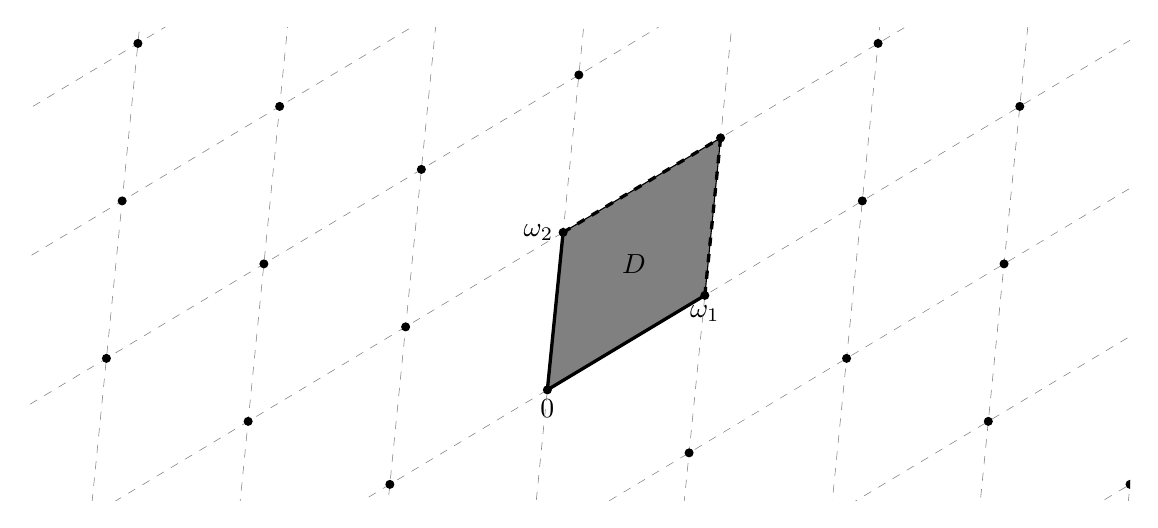
\begin{tikzpicture}
        \begin{scope}
            \clip (0,0) rectangle (14cm,6cm); % Clips the picture...
            \pgftransformcm{1}{0.6}{0.1}{1}{\pgfpoint{3cm}{3cm}} % This is actually the transformation
            %  matrix entries that gives the slanted
            % unit vectors. You might check it on
            % MATLAB etc. . I got it by guessing.
            
            \draw (4,-2) node [left]{$\omega_2$};
            \draw (4,-4) node [below]{$0$};
            \draw (6,-4) node [below]{$\omega_1$};
            \draw[style=help lines,dashed] (-14,-14) grid[step=2cm] (18,14); % Draws a grid in the new coordinates.
            \filldraw[fill=gray, draw=black] (4,-4) rectangle (6,-2); % Puts the shaded rectangle
            \draw[black, very thick] (4,-4) -- (6,-4);
            \draw[black, very thick] (4,-4) -- (4,-2);
            \draw[black, very thick, dashed] (4,-2) -- (6,-2);
            \draw[black, very thick, dashed] (6,-4) -- (6,-2);

            \draw (5,-3) node {$D$};
            \foreach \x in {-7,-6,...,8}{                           % Two indices running over each
            \foreach \y in {-7,-6,...,8}{                       % node on the grid we have drawn 
            \node[draw,circle,inner sep=1pt,fill] at (2*\x,2*\y) {}; % Places a dot at those points
            }
            }
        \end{scope}
    \end{tikzpicture}

    \caption{Mreža.}
    \label{mreza}
\end{figure}

Na kompleksno ravnino $\C$ vpeljimo relacijo 
\[
    z \sim w \iff z - w \in \Lambda \quad \text{ za vsaka $z,w \in \C$.}
\]
To pomeni, da identificiramo vsaki dve točki, ki se razlikujeta kvečjemu za prišteto periodo $\omega \in \Lambda$. 
Brez težav se lahko prepričamo, da je to ekvivalenčna relacija na $\C$. Tako lahko tvorimo kvocientno množico $\C/_{\sim}$, katere ekvivalenčne razrede bomo označevali z $z + \Lambda$ in jih imenovali \emph{translati}, saj si jih lahko predstavljamo kot za vektor $z$ translirano mrežo $\Lambda$. Pripadajoča kvocientna projekcija bo $\pi : \C \to \C/_{\sim}$. Kvocient $\C/_{\sim}$ bomo od tod dalje rajši označevali z $\C/\Lambda$. 

Zaenkrat bomo $\C/\Lambda$ razumeli zgolj kot kvocientno množico, kasneje pa ga bomo opremili s topologijo, ki nam bo razkrila, da je ta prostor v resnici homeomorfen torusu. Za tem bomo definirali še s kompleksno strukturo, ki nam bo na njem omogočila definirati holomorfne preslikave.


\begin{definicija}
    \emph{Fundamentalni paralelogram} za mrežo $\Lambda = \langle \om_1, \om_2 \rangle$ je
    \[
        D_{\alpha} = \{\alpha + t_1 \om_1 + t_2 \om_2 \mid t_1, t_2 \in [0,1)\}.
    \]
    Zaprtje fundamentalnega paralelograma $D_\alpha$ v $\C$ bomo označili z $\ols{D}_\alpha$. 
\end{definicija}

\begin{opomba}
    Kadar bomo govorili o fundamentalnih domenah pogosto izbira izhodišča $\alpha$ ne bo pomembna, zato ga bomo tedaj izpustili in pisali samo $D$. V tem primeru lahko privzamemo, da je s tem mišljen $D_0$. 
\end{opomba}

Naslednja lema pove, da je preslikava $D_\alpha \to \C/\Lambda$ bijekcija med možicama. 

\begin{lema}
    \label{enolicni predstavnik}
    Poljuben translat $z + \Lambda$ mreže $\Lambda \subseteq \C$ ima natanko enega predstavnika v fundamentalni domeni $D_\alpha$. 
\end{lema}

\begin{dokaz}
    Ker sta osnovni periodi $\omega_1, \omega_2$ $\R$-linearno neodvisni, tvorita bazo za $\C$ gledano kot realen vektorski prostor. Tako lahko zapišemo $z - \alpha = a_1 \om_1 + a_2 \om_2$, kjer sta $a_1, a_2 \in \R$. Tedaj za 
    \[
        t_i = a_i - \lfloor a_i \rfloor \in [0,1) \quad \text{ za $i \in \{1,2\}$},
    \] 
    kjer $\lfloor x \rfloor$ označuje največje celo število, ki ni večje od $x$, velja $\alpha + t_1\om_1 + t_2 \om_2 = z - \lfloor a_1 \rfloor \om_1 - \lfloor a_2 \rfloor \om_2 \in D_\alpha \cap (z + \Lambda)$.
\end{dokaz}

Spomnimo se, da so \emph{holomorfne} funkcije na neki odprti domeni $D$ tiste, ki jih je mogoče odvajati v kompleksnem smislu povsod na $D$. Kolobar holomorfnih funkcij na $D$ označimo z $\hol{D}$. Če je funkcija holomorfna na celotnem $\C$, pravimo, da je \emph{cela holomorfna} funkcija. Te označimo z $\hol{\C}$.

Če je $S \subseteq D$ diskretna množica brez stekališč v $D$, potem funkcijam, ki so holomorfne na $D \setminus S$ v točkah iz $S$ pa imajo pole, pravimo \emph{meromorfne} funkcije, točkam iz $S$ pa \emph{singularnosti}. Vsako meromorfno funkcijo $f$ na $D \subseteq \C$, lahko vidimo tudi kot preslikavo $D \to \RS$, kjer dodatno definiramo 
\[
    f(w) = \infty \quad \text{za vsak $w \in S$.} 
\]

\begin{definicija}
    Naj bo $f$ meromorfna funkcija na $\C$ in $\Lambda \subseteq \C$ mreža. Če za $f$ velja
    \[
        f(z + \om) = f(z) \quad \text{za vse $\om \in \Lambda$ in $z \in C$},
    \]
    potem pravimo, da je $f$ \emph{eliptična} oziroma \emph{dvojno periodična} funkcija. Kadar želimo poudariti, da je $f$ eliptična glede na mrežo $\Lambda$, pravimo, da je \emph{$\Lambda$-periodična}. Polje $\Lambda$-periodičnih funkcij označimo z $\C(\Lambda)$. % mogoče tega zadnjega ne rabim
\end{definicija}




%%%%% Lastnosti eliptičnih funkcij %%%%%

\subsection{Lastnosti eliptičnih funkcij}

Sedaj si bomo pogledali nekaj izrekov, ki opisujejo naravo eliptičnih funkcij in jih lahko povečini priprišemo Liouvillu. Prvi je direktna posledica njegovega slavnega izreka iz kompleksne analize, ki pove, da razen konstant celih omejenih holomorfnih funkcij ni. Bralec ga lahko najde v \cite[]{}.

\begin{izrek}
    \label{cele el. funkcije}
    Naj bo $f$ cela eliptična funkcija. Tedaj je $f$ konstantna.
\end{izrek}

\begin{dokaz}
    Ker je $f$ konstantna na ekvivalenčnih razredih množice $\C/\Lambda$ tj. translatih oblike $z + \Lambda$, je enolično določena že z vrednostjo na enem od predstavnikov vsakega translata. Po lemi \ref{enolicni predstavnik} vidimo, da lahko predstavnika poljubnega translata najdemo v fundametnalnem paralelogramu $D$, zato bo 
    \[
        \sup_{z \in \C} \left\lvert f(z) \right\rvert = \sup_{z \in \olsi{D}} \left\lvert f(z) \right\rvert.
    \]
    % $f$ tako enolično določena že z vrednostmi na $D$. 
    Ker je $f$ holomorfna na celotnem $\C$, je tam seveda zvezna in je zato zvezna tudi na zaprtju fundamentalnega paralelograma $\olsi{D}$. To je zaprta in omejena množica v $\C$ in je tako kompaktna \cite[Trditev 2.22]{MrcunTop}. Zvezna funkcija $f$ je na kompaktu $\olsi{D}$ omejena, kot eliptična funkcija pa je tako omejena na celotnem $\C$ \cite[Posledica 2.28]{MrcunTop}. Funkcija $f$ je torej omejena in cela holomorfna, zato je po Liouvillovem izreku konstantna.  
\end{dokaz}

\begin{opomba}
    Enako lahko sklepamo tudi, če $f$ nima ničel. Tedaj je $1/f$ cela eliptična funkcija, ko jo v polih $f$ razširimo z $0$.
\end{opomba}

\begin{lema}
    \label{odvod el. funkcije}
    Naj bo $f \in \elf$ eliptična funkcija. Tedaj je tudi njen odvod $f' \in \elf$ eliptična funkcija.
\end{lema}

\begin{dokaz}
    Recimo, da je $z \in \C$ točka, kjer $f$ nima pola, zato je v njeni okolici holomorfna in jo lahko odvajamo v kompleksnem smislu. Z odvajanjem osnovnega pogoja za eliptične funkcije dobimo
    \[
        f'(z + \omega) = f'(z) \quad \text{ za vsak $\omega \in \Lambda$.}
    \]
    Če je v točki $z \in \C$ pol, pa ima tudi $f'$ v tej točki pol, torej pogoj za eliptičnost velja povsod na $\C$ in tako je $f' \in \elf$.
\end{dokaz}

Vpeljimo nekaj notacije, ki jo bomo potrebovali v naslednjih izrekih. Če je $f$ meromorfna funkcija na odprti domeni $D \subseteq \C$, pravimo, da je $f$ \emph{reda $m \in \Z$} v točki $z_0 \in D$, če obstaja okolica $U \subseteq D$ točke $z_0$ in holomorfna funkcija $g \in \hol{U}$, ki je neničelna povsod na $U$, da velja 
\[
    f(z) = (z - z_0)^m g(z) \quad \text{za vse $z \in U$.}  
\]   
Tedaj označimo $\ord{z_0}{f} = m$. Če je $m > 0$ ima $f$ v $z_0$ \emph{ničlo} reda $m$, če pa je $m < 0$ ima $f$ v $z_0$ \emph{pol} reda $-m$.

\emph{Residuum} ali \emph{ostanek} funkcije $f$ pri točki $z_0 \in D$, je koeficient pred potenco $(z-z_0)\inv$ v Laurentovi vrsti za $f$ okrog $z_0$. Označimo ga z $\res{z_0}{f}$. 

% \begin{komentar}
%     Z $\sum_{w \in \torus}$ bomo označili vsoto po $w \in D$ poljubnem fundamentalnem paralelogramu, ki pripada merži $\Lambda$ in katerega rob ne vsebuje ničel ali polov funkcije $f$.   
% \end{komentar}

\begin{izrek}
    \label{liouville}
    Naj bo $f \in \C(\Lambda)$ eliptična funkcija in $D$ fundamentalni paralelogram glede na mrežo $\Lambda$, katerega rob $\partial D$ ne vsebuje polov ali ničel $f$. Tedaj velja
    \begin{flalign*}
        &\sum_{w \in D} \res{w}{f} = 0 && \label{identiteta 1} \tag{a} \\ 
        &\sum_{w \in D} \ord{w}{f} = 0 && \label{identiteta 2} \tag{b} \\
        &\sum_{w \in D} \ord{w}{f}\cdot w \in \Lambda. && \label{identiteta 3} \tag{c}
    \end{flalign*}

    % \begin{enumerate}[(a)]
    %     \item \[\sum_{w \in D} \res{w}{f} = 0\] \label{identiteta 1}
    %     \item \[\sum_{w \in D} \ord{w}{f} = 0\] \label{identiteta 2}
    %     \item \[\sum_{w \in D} \ord{w}{f}\cdot w \in \Lambda.\] \label{identiteta 3}
    % \end{enumerate}    
\end{izrek}

\begin{dokaz}
    \par
    (\ref{identiteta 1}) Uporabimo izrek o ostankih \cite[Izrek 71]{Globevnik}, ki pove
    \[
        \sum_{w \in D} \res{w}{f} = \frac{1}{2\pi i}\int_{\partial D} f(z)dz.  
    \]
    Razdelimo rob fundametalnega paralelograma $\partial D = \sigma_1 \cup \sigma_2 \cup \sigma_3 \cup \sigma_4$ na štiri daljice, ki ga omejujejo, kot prikazuje slika \ref{fundamentalni paralelogram}.

    \begin{figure}[H]
        \centering
        
\begin{tikzpicture}
            \begin{scope}
                \clip (0,0) rectangle (14cm,4cm); % Clips the picture...
                \pgftransformcm{1}{0.6}{0.1}{1}{\pgfpoint{2cm}{2cm}};
                \filldraw[fill=gray, draw=black] (4,-4) rectangle (6,-2);
                % \draw (4,-2) node [left]{$\alpha + \omega_2$};
                \draw (4,-4) node [below]{$\alpha$};
                % \draw (6,-4) node [below]{$\alpha + \omega_1$};
                \draw (5,-3) node {$D$};
                \draw (4,-3) node [left]{$\sigma_4$};
                \draw (5,-4) node [below]{$\sigma_1$};
                \draw (6,-3) node [right]{$\sigma_2$};
                \draw (5,-2) node [above]{$\sigma_3$};
                
                \foreach \x in {4,6}{                          
                    \foreach \y in {-4,-2}{                       
                        \node[draw,circle,inner sep=1pt,fill] at (\x,\y) {}; 
                    }
                }
                
            \end{scope}
        \end{tikzpicture}
        
        \caption{Fundamentalni paralelogram.}
        \label{fundamentalni paralelogram}
    \end{figure}


    Jasno tedaj velja
    \[
        \int_{\partial D} f(z)dz = \int_{\sigma_1} f(z)dz + \int_{\sigma_2} f(z)dz + \int_{\sigma_3} f(z)dz + \int_{\sigma_4} f(z)dz,
    \]
    s preprosto zamenjavo spremenljivk pa je zaradi periodičnosti $f$ preprosto videti, da se integrala po nasprotnih stranicah odštejeta, kar nam da želeni rezultat. 
    \\
    \par
    (\ref{identiteta 2}) Po lemi \ref{odvod el. funkcije} je $f' \in \elf$, zato je tudi kvocient $f'/f \in \elf$ eliptičen. Tedaj velja
    \[
        \sum_{w \in D} \ord{w}{f} = \frac{1}{2\pi i}\int_{\partial D} \frac{f'(z)}{f(z)}dz = 0. 
    \]
    Kjer smo v prvi enakosti uporabili princip argumenta \cite[Izrek 72]{Globevnik}, druga enakost pa je identiteta (\ref{identiteta 1}), ki velja zaradi eliptičnosti $f'/f$.
    \\
    \par
    % mogoče bom povsod zamenjal $z_0$ z $w$...
    (\ref{identiteta 3}) Oglejmo si funkcijo $z \mapsto z \frac{f'(z)}{f(z)}$. Jasno je ta funkcija meromorfna na $\C$. Naj bo $z_0 \in \C$ poljuben. Tedaj obstaja $m \in \Z$, okolica $U \subseteq \C$ točke $z_0$ in holomorfna funkcija $g \in \hol{U}$, ki je neničelna na $U$, da velja
    \[
        f(z) = (z - z_0)^m g(z) \quad \text{ za vsak $z \in U$.}  
    \]
    Z odvajanjem te enakosti dobimo
    \[
        f'(z) = m(z - z_0)^{m - 1} g(z) + (z - z_0)^m g'(z),
    \]
    ki pravtako velja povsod na $U$. Skupaj tako dobimo, da za vsak $z \in U$ velja
    \[
        z\frac{f'(z)}{f(z)} = \frac{mz}{z-z_0} + z\frac{g'(z)}{g(z)} = \frac{mz_0}{z-z_0} + \underbrace{m + z\frac{g'(z)}{g(z)}}_{\in \hol{U}}.
    \]
    Ker sta zadnja dva člena holomorfna na $U$, edino člen $\frac{mz_0}{z-z_0}$ prispeva h glavnemu delu Laurentovega razvoja funkcije $z \mapsto z \frac{f'(z)}{f(z)}$ okrog $z_0$. Zato je 
    \[
        \operatorname{res}_{z_0} \left( z \frac{f'(z)}{f(z)} \right) = mz_0 = \ord{z_0}{f}z_0.  
        % \res{z_0}{z \frac{f'(z)}{f(z)}} = mz_0 = \ord{z_0}{f}z_0.  
    \]
    Tako dobimo 
    \[
        \sum_{w \in D} \ord{w}{f}\cdot w 
        = \sum_{w \in D} \operatorname{res}_{w} \left( z \frac{f'(z)}{f(z)} \right)
        = \frac{1}{2 \pi i} \int_{\partial D} z \frac{f'(z)}{f(z)}dz. 
    \] 
    Poglejmo si sedaj zadnji integral, ki ga podobno kot pri dokazu (\ref{identiteta 1}) razbijemo na vsoto integralov po štirih stranicah. Argument o odštevanju integralov po nasprotnih stranicah paralelograma pa tokrat zaradi neperiodičnosti funkcije $z \mapsto z \frac{f'(z)}{f(z)}$ ne bo deloval. Z uvedbo nove spremenljivke $w = z + \omega_2$ v integral po stranici $\sigma_1$ vidimo
    \begin{multline*}
        \int_{\sigma_1} z \frac{f'(z)}{f(z)}dz = 
        \int_{\sigma_1} z \frac{f'(z + \omega_2)}{f(z + \omega_2)}dz = \\ = 
        - \int_{\sigma_3} (w - \omega_2) \frac{f'(w)}{f(w)}dw = 
        - \int_{\sigma_3} z \frac{f'(z)}{f(z)}dz + \omega_2 \int_{\sigma_3} \frac{f'(z)}{f(z)}dz.
    \end{multline*}
    Podobno z uvedbo nove spremenljivke $w = z + \omega_1$ storimo z integralom po stranici $\sigma_2$ in tako dobimo
    \[
        \int_{\partial D} z \frac{f'(z)}{f(z)}dz = \omega_1 \int_{\sigma_4} \frac{f'(z)}{f(z)}dz + \omega_2 \int_{\sigma_3} \frac{f'(z)}{f(z)}dz.
    \]
    \\

    Za poljubno sklenjeno in kosoma gladko krivuljo $\gamma : [0,1] \to \C$, tj. $\gamma(0) = \gamma(1)$, ki ne poteka skozi izhodišče $0\in \C$, je
    \[
        \frac{1}{2 \pi i} \int_\gamma \frac{dz}{z} \in \Z
    \]
    \emph{ovojno število} krivulje $\gamma$ okoli $0$ in nam pove kolikokrat se krivulja $\gamma$ ovije okoli izhodišča. Podrobnosti o tem lahko bralec najde v \cite[4.2.1.]{Ahlfors}.
    \\

    Osredotočimo se sedaj samo na prvi integral, premislek za drugega je analogen. Opazimo, da je zaradi eilptičnosti $f$ krivulja $f(\sigma_4)$ sklenjena, saj sta krajišči daljice $\sigma_4$ točki $\alpha$ in $\alpha + \omega_2$ v katerih ima $f$ enaki vrednosti. Pot $\gamma : [0,1] \to f(\sigma_4)$, ki predstavlja to sklenjeno krivuljo, je podana s predpisom $t \mapsto f(\alpha + t\omega_2)$. Opomnimo še, da to ni nujno parametrizacija krivulje v običajnem smislu, saj je lahko neinjektivna. 
    
    Zapišemo lahko 
    \[
        2 \pi i k_1 = 
        \int_{\gamma} \frac{dz}{z} = 
        \int_0^1 \frac{\gamma'(t)}{\gamma(t)}dt =
        \int_0^1 \frac{f'(\alpha + t\omega_2)}{f(\alpha + t\omega_2)}\omega_2 dt = 
        \int_{\sigma_4} \frac{f'(z)}{f(z)}dz
    \]
    za nek $k_1 \in \Z$. Podobno je tako tudi
    \[
        2 \pi i k_2 = \int_{\sigma_3} \frac{f'(z)}{f(z)}dz,
    \]
    za nek $k_2 \in \Z$. Skupaj je torej 
    \[
        \sum_{w \in D} \ord{w}{f} \cdot w = 
        \frac{1}{2 \pi i} \int_{\partial D} z\frac{f'(z)}{f(z)}dz = 
        k_1 \omega_1 + k_2 \omega_2\in \Lambda.  
    \]
\end{dokaz}

\begin{opomba}
    \label{liouville opomba}
    \begin{enumerate}
        \item
        V vseh treh točkah seštevamo po neštevnem fundamentalnem paralelogramu $D$, toda vse tri vsote vsebujejo zgolj končno mnogo neničelnih členov. Residuum in red funkcije $f$, sta lahko različna od nič samo v ničlah ali polih $f$, teh pa je v kompaktu $\ols{D}$ lahko le končno, saj bi sicer prišli v protislovje s principom identičnosti. Ta pravi, da se meromorfni funkciji definirani na neki odprti domeni $\Omega$, ki se ujemata na množici s stekališčem v $\Omega$, ujemata povsod na $\Omega$ \cite[]{}.
        \item 
        Kot nakazuje izrek je izbira fundamentalnega paralelograma irelevantna, dokler ta izpolnjuje določene predpostavke o robu. Kljub temu pa se prepričajmo, da lahko vselej takšen fundamentalni paralelogram vedno izberemo. 

        Denimo, da temu ni tako, torej da ima vsak fundamentalni paralelogram na svojem robu vsaj en pol eliptične funkcije $f$. S translacijami
        \[
            \tau_n : z \mapsto z + \frac{1}{n}(\om_1 + \om_2); \quad n\in \N
        \]
        delujemo na rob fundamentalnega paralelograma $\partial D$ in tako dobimo števno mnogo različnih polov za $f$. To zaporedje polov leži v uniji $\cup_{n \in \N} \tau_n(\partial D)$, ki jo lahko zapremo v dovolj velik zaprt disk. Na ta način dobimo zaporedje polov v kompaktu, ki ima po Bolzano-Weierstrassovem izreku stekališče, kar pa je v nasprotju s tem, da je množica polov meromorfne funkcije diskretna v $\C$. 
        
        Podobno lahko hkrati sklepamo še za ničle funkcije $f$ in s pomočjo principa identičnosti pridemo v protislovje z diskretnostjo množice ničel meromorfne funkcije $f$.
        \item 
        Točka (\ref{identiteta 2}) pove, da ima eliptična funkcija na fundamentalnem paralelogramu enako število ničel in polov štetih z večkratnostjo. 
    \end{enumerate}
\end{opomba}

\begin{definicija}
    \emph{Red} eliptične funkcije je število polov šteto z večkratnostjo v poljubnem fundamentalnem paralelogramu. 
\end{definicija}

Tudi, če pol $z_0$ leži na robu $\partial D$ izbranega fundamentalnega paralelograma, lahko govorimo o redu tega pola v $D$. Takrat štejemo \emph{red pola $z_0$ v $D$} kot $\frac{1}{2}\ord{z_0}{f}$, če pol ni eno od štirih oglišč, oziroma, v primeru ko pol $z_0$ je oglišče paralelograma, vzamemo za njegov red vrednost
\[
    \frac{\ell(\partial \Delta(z_0, r) \cap D)}{2 \pi r}\ord{z_0}{f}.
\]
Ob tem $\ell$ opisuje dolžino danega krožnega loka, $r > 0$ pa je dovolj majhen, da je $z_0$ edino oglišče fundamentalnega paralelograma vsebovano v odprtem disku ${\Delta(z_0, r) =}$ ${\{z \in \C \mid \left\lvert z - z_0 \right\rvert < r\}}$. Z drugimi besedami je ta količina normaliziran notranji kot fundamentalnega paralelograma pri oglišču $z_0$ pomnožen z $\ord{z_0}{f}$.  

\begin{zgled*}

\end{zgled*}

\begin{posledica}
    Nekonstantna eliptična funkcija ima red vsaj $2$.
\end{posledica}

\begin{dokaz}
    Denimo, da je $f \in \elf$ eliptična funkcija z enim polom na fundamentalni domeni $D$, saj vemo že, da bi bila konstantna, če nebi imela nobenega pola po izreku \ref{cele el. funkcije}. Brez škode za splošnost lahko predpostavimo, da pol leži v notranjosti $D$. Tedaj dobimo z integracijo po robu $\partial D$ neničelni residuum
    \[
        0 \neq \res{\alpha}{f} = \frac{1}{2 \pi i} \int_{\partial D} f(z)dz.  
    \]
    To pa je v nasprotju z izrekom \ref{liouville} (\ref{identiteta 1}), ki pove, da je ta residuum -- edini člen v vsoti -- enak nič. 
\end{dokaz}

\begin{posledica}
    Nekonstantna eliptična funkcija $f: \C \to \RS = \C \cup \{\infty\}$ je surjektivna. 
\end{posledica}

\begin{dokaz}
    Ker je $f \in \elf$ nekonstantna, ima po izreku \ref{cele el. funkcije} pol in lahko zato rečemo, da tam doseže točko $\infty$. Naj bo sedaj $w \in \C$ poljubna točka in pokažimo, da obstaja $z \in \C$, da velja $f(z) = w$.
    
    Definirajmo $g(z) := f(z) - w$. Funkcija $g$ je pravtako eliptična in ima pol, saj je takšna $f$ in prištevanje konstante na ti dve lastnosti nima vpliva. Po opombi \ref{liouville opomba} (3) ima $g$ ničlo v $\C$, kar pokaže želeno.
\end{dokaz}



%%%%% Weierstrassova funkcija %%%%%

\subsection{Weierstrassova funkcija $\wp$}

Osrednja tema tega poglavja, ki bo povezala eliptične krivulje s kompleksnimi torusi in za katero je bilo potrebno razvijati teorijo v prejšnjem razdelku, bo t.~i.\ \emph{Weierstrassova funkcija} $\wp$. 

Vseskozi naj bo $\Lambda$ mreža v $\C$ in naj velja oznaka $\Lambda' = \Lambda \setminus \{0\}$.

\begin{definicija}
    \label{eisensteinova vrsta}
    Za celo število $k > 2$ je \emph{Eisensteinova vrsta reda $k$} podana kot
    \[
        G_k(\Lambda) = \sum_{\om \in \Lambda'} \frac{1}{\om^k}.  
    \]
\end{definicija}

\begin{opomba}
    Opazimo, da za lihe $k$ velja $G_k(\Lambda) = 0$, saj se člena pri $\om$ in $-\om\in\Lambda'$ v vsoti odštejeta. 
\end{opomba}

\begin{lema}
    \label{lema o konvergenci eisensteinove vrste}
    Za vsako celo število $k > 2$ Eisensteinova vrsta reda $k$ absolutno konvergentna.
\end{lema}

\begin{dokaz}
    Za vsak $n \in \N$ definirajmo množice
    \[
        C_n = \{k_1 \om_1 + k_2 \om_2\in \Lambda \mid k_1 + k_2 = n\}.  
    \]
    Preprosto se je prepričati, da je moč posamezne od teh množic $\#C_n = 4n$. Vsak element $\om \in C_n$ pa lahko po absolutni vrednosti ocenimo $\left\lvert \om \right\rvert > \rho n$, kjer je $\rho > 0$ razdalija od izhodišča $0$, do roba paralelograma z oglišči v točkah $\pm \om_1, \pm \om_2$. Tedaj velja ocena
    \[
        \sum_{\om \in \Lambda'} \frac{1}{\left\lvert  \om^k \right\rvert} = 
        \sum_{n = 1}^\infty \sum_{\om \in C_n} \frac{1}{\left\lvert  \om \right\rvert^k} \leq
        \sum_{n = 1}^\infty \sum_{\om \in C_n} \frac{1}{(\rho n)^k} =
        \sum_{n = 1}^\infty \frac{4n}{\rho^k n^k} = 
        \frac{4}{\rho^k} \sum_{n = 1}^\infty \frac{1}{n^{k-1}}.
    \]
    Zadnja vrsta konvergira natanko tedaj, ko je $k - 1 > 1$ in tako po primerjalnem kriteriju dobimo absolutno kovergenco vrste $\sum_{\om \in \Lambda'} \om^{-k}$.
\end{dokaz}

\begin{lema}
    \label{elipticna vrsta}
    Za vsako celo število $k > 2$, vrsta 
    \[
        \sum_{\om \in \Lambda'} \frac{1}{(z - \om)^k}
    \]
    konvergira absolutno za poljuben $z\in \C\setminus\Lambda'$ in enakomerno po kompaktih na $\C \setminus \Lambda'$. 
\end{lema}

\begin{dokaz}
    Glavna ideja dokaza bo s pomočjo nekaj ocen uporabiti Weierstrassov M-test. Naj bo $K \subseteq \C$ poljuben kompakt disjunkten z $\Lambda'$. Kot tak je omejen, zato je vsebovan v nekem disku $\Delta(0,r)$ z radijem $r > 0$. Razdelimo obravnavo period $\omega \in \Lambda'$ na tiste, ki ležijo v disku $\Delta(0,2r)$ in na tiste, ki ne.
    
    (i) Za vse $\omega \in \Lambda' \cap \Delta(0,2r)$ zaradi kompaktnosti $K$ obstaja
    \[
        \min_{z \in K} \abs{z - \omega} =: \epsilon_\omega > 0
    \]
    Ker pa je takšnih period, za katere je $\abs{\omega} < 2r$, zgolj končno mnogo, denimo $n \in \N$, lahko za $\epsilon$ izberemo najmamnjšega izmed $\epsilon_\om$ in tako velja 
    \[
        \abs{z - \omega} \geq \epsilon \quad \text{za vse $z \in K$ in vse $0 < \abs{\omega} < 2r$.}  
    \]
    
    (ii) Za vse periode $\abs{\omega} \geq 2r$ pa preko trikotniške neenakosti
    \[
        \abs{\om} \leq \abs{z - \om} + \abs{z} \quad \text{za vse $z \in K$}
    \]
    vidimo, da velja 
    \[
        \abs{z - \om} \geq 
        \abs{\om} - \abs{z} \geq 
        \abs{\om} - r \geq 
        \abs{\om} - \frac{1}{2}\abs{\om} \geq
        \frac{1}{2}\abs{\om} \quad \text{za vse $z\in K$.}
    \]
    Tako pridemo do ocene
    \[
        \sum_{\om \in \Lambda'} \frac{1}{\abs{z - \om}^k} = 
        \sum_{\substack{\om \in \Lambda' \\ \abs{\om} < 2r}} \frac{1}{\abs{z - \om}^k} + \sum_{\substack{\om \in \Lambda' \\ \abs{\om} \geq 2r}} \frac{1}{\abs{z - \om}^k} \leq
        \frac{n}{\epsilon^k} + \sum_{\substack{\om \in \Lambda' \\ \abs{\om} \geq 2r}} \frac{2^k}{\abs{\om}^k},
    \]
    ki velja povsod na $K$. Ker je zadnja vsota del absolutno konvergentne Eisensteinove vrste reda $k$ po lemi \ref{lema o konvergenci eisensteinove vrste}, nam Weierstrassov M-test zagotavlja želeni rezultat.
\end{dokaz}

\begin{izrek}
    Naj bo $(f_n)_{n \in \N}$ zaporedje holomorfnih funkcij na odprti domeni $\Omega \subseteq \C$, ki enakomerno po kompaktih v $\Omega$ konvergira k limitni funkciji $f$. Tedaj je tudi $f \in \hol{\Omega}$ holomorfna na $\Omega$ in zaporedje odvodov $(f'_n)_{n\in \N}$ konvergira enakomerno po kompaktih k odvodu limitne funkcije $f'$.
\end{izrek}

\begin{dokaz}
    \cite[\S 5, Theorem 1]{Ahlfors}
\end{dokaz}
    
% Kot preslikava $\C \to \RS$ vrsta 
% \[
%     \sum_{\om \in \Lambda} \frac{1}{(z - \om)^k}
% \]
% zaradi enakomerne konvergence po kompaktih v $\C\setminus\Lambda$ predstavlja meromorfno funkcijo s poli v možici $\Lambda'$. 


% \begin{dokaz}
%     Glavna ideja tukaj bo uporabiti Weierstrassov M-test. Najprej pa si pripravimo oceno. 
    
%     Naj bo $K\subseteq \C\setminus \Lambda'$ poljuben kompakt. Kot kompakt v evklidskem prostoru je omejen, torej obstaja $r > 0$, da je $K \subseteq \Delta(0,r)$. Za vseh razen končno mnogo $\omega\in\Lambda$, ki ležijo v disku $\Delta(0,2r)$, velja 
%     \[
%         \abs{\omega} \geq 2r \geq 2\abs{z} \quad \text{za vsak $z\in K$,}
%     \] 
%     od tod pa preko trikotniške neenakosti $\abs{\omega} \leq \abs{z - \omega} + \abs{z}$ dobimo 
%     \begin{equation}
%         \label{ocena za vrsto}
%         \abs{z - \om} \geq \abs{\om} - \abs{z} \geq \frac{1}{2}\abs{\om} \quad \text{za vse $z \in K$ in $\abs{\om} \geq 2r$.}  
%     \end{equation}
%     % Za teh končno mnogo $\omega \in \Delta(0,2r)\cap \Lambda$ pa obstaja konstanta $c>0$, da velja
%     % \[
%     %     \abs{z - \om} \geq c \quad \text{za vse $z \in K$.}  
%     % \] 

%     Sedaj definirajmo funkcijsko zaporedje $(f_n)_{n \in \N}$ na $K$ podano kot
%     \[
%         f_n(z) = \sum_{\substack{\om\in\Lambda' \\ 2r \leq \abs{\om} < n}} \frac{1}{(z - \om)^k}.
%     \]
%     Zanj velja
%     \[
%         \abs{f_n(z)} \leq 
%         \sum_{\substack{\om\in\Lambda' \\ 2r \leq \abs{\om} < n}} \frac{1}{\abs{z - \om}^k} \leq
%         \sum_{\substack{\om\in\Lambda' \\ 2r \leq \abs{\om} < n}} \frac{2^k}{\abs{\om}^k} \leq
%         \sum_{\om\in\Lambda'} \frac{2^k}{\abs{\om}^k},
%     \]
%     kjer smo za drugo neenakost uporabili oceno \ref{ocena za vrsto}. Vrsta na desni konvergira kot smo ugotovili v dokazu leme \ref{lema o oceni vrste po mrezi}, tako pa nam je uspelo funkcijsko zaporedje $(f_n)_{n\in \N}$ po absolutni vrednosti navzgor omejiti s konstantnim -- torej konvergentnim zaporedjem. Po Weierstrassovem M-testu \cite[]{Globevnik} je funkcijsko zaporedje $(f_n)_{n\in \N}$ absolutno in enakomerno konvergentno na poljubem kompaktu $K \subseteq \C\setminus\Lambda'$.
    
%     Enako torej velja tudi za vrsto 
%     \[
%         \sum_{\om \in \Lambda'} \frac{1}{(z - \om)^k} = 
%         \sum_{\substack{\om \in \Lambda' \\ \abs{\om} < 2r}} \frac{1}{(z - \om)^k} + \lim_{n \to \infty} f_n(z).
%     \]
%     % te delne vsote pa bomo za dovolj velike $n\in\N$ poskusili omejiti s členom konvergentnega zaporedja, ki je neodvisno od $z \in K$. Za majhne $n\in \N$, torej tiste za katere je $n < r$, pa že imamo oceno 
%     % \[
%     %     \abs{f_n(z)} = \sum_{\substack{\om\in\Lambda' \\ n-1 \leq \abs{\om} < n}} \frac{1}{\abs{z - \om}^s} \leq \frac{}{c^s}
%     % \]
%     % ki je neodvisna od $z\in K$.  
% \end{dokaz}

\begin{primer*}
    Tako smo prišli, do prvega netrivialnega primera eliptične funkcije. Prepričajmo se, da je funkcija podana s predpisom
    \[
        f(z) = \sum_{\om \in \Lambda} \frac{1}{(z - \om)^k}, \quad \text{za k > 2}  
    \]
    res ne le meromorfna, ampak tudi eliptična (to je vrsta iz leme \ref{elipticna vrsta}, ki smo ji prišteli člen $z^{-k}$).

    Če je $z \in \C$ poljuben in $\om_0 \in \Lambda$ poljubna perioda, računamo
    \[
        f(z + \om_0) = 
        \sum_{\om \in \Lambda} \frac{1}{(z + \om_0 - \om)^k} = 
        \sum_{\om \in \Lambda} \frac{1}{(z - (\om - \om_0))^k} = 
        \sum_{\om \in \Lambda} \frac{1}{(z - \om)^k} = 
        f(z),
    \]
    kjer smo v predzadnji enakosti upoštevali, da je translacija $\om \mapsto \om - \om_0$ bijekcija mreže $\Lambda$ samo vase, ki nam zgolj premeša vrstni red seštevanja v zadnji vsoti. 
\end{primer*}


\break




%--------------------------------------------------------------------------%
%%%%%%%%%%%%%%%%%%%%%%% 4. RIEMANNOVE PLOSKVE %%%%%%%%%%%%%%%%%%%%%%%%%%%%%%
%--------------------------------------------------------------------------%

\section{Riemannove ploskve} \label{riemannove ploskve}
\subsection{Definicije in lastnosti}
\subsection{Kompleksna struktura na eliptični krivulji}
\subsection{Kompleksna struktura na torusu}
\break


%--------------------------------------------------------------------------%
%%%%%%%%%%%%%%%%%%%%%%%%%%% 5. IZOMORFIZEM %%%%%%%%%%%%%%%%%%%%%%%%%%%%%%%%%
%--------------------------------------------------------------------------%


\section{Izomorfizem \texorpdfstring{$\C/\Lambda \to E(\C)$}{} in njegove posledice} \label{poglavje izomorfizem}

\subsection{Uniformizacija}
\subsection{$j$-invarianta}
 
% koeficienta 60 in 140 pred G_4, G_6 sta najmanjša, da je ena limita v zvezi z diskriminanto enaka 0...

\break

\section*{Slovar strokovnih izrazov}

\geslo{}{}
\geslo{}{}

% seznam uporabljene literature

% (!) urejen po abecednem vrstenm redu priimkov avtorjev 
\begin{thebibliography}{99}
    
    \bibitem{Ahlfors}
        L.~V.~Ahlfors, \emph{Complex analysis}, third edition, McGraw-Hill, Inc., New York, 1979.

    \bibitem{Gibson}
        C.~G.~Gibson, \emph{Elementary geometry of algebraic curves: An undergraduate introduction}, Cambridge University Press, Cambridge, 1998.

    \bibitem{Globevnik}
        J.~Globevnik in M.~Brojan, \emph{Analiza II}, verzija 10.~8.~2010, [ogled 28.~7.~2021], dostopno na \url{https://www.fmf.uni-lj.si/~globevnik/skriptaII.pdf}.
    
    \bibitem{LangEllfunc}
        S.~Lang, \emph{Elliptic functions}, Graduate Texts in Mathematics \textbf{112}, Springer-Verlag, New York, 1973.

    \bibitem{MrcunTop}
        J.~Mrčun, \emph{Topologija}, Izbrana poglavja iz matematike in računalništva \textbf{44}, DMFA--založništvo, Ljubljana, 2008.
    
    \bibitem{Silverman}
        J.~H.~Silverman, \emph{The arithmetic of elliptic curves}, Graduate Texts in Mathematics \textbf{106}, Springer-Verlag, New York, 1986.

    \bibitem{Stevenhagen}    
        P.~Stevenhagen, \emph{Complex elliptic curves}, verzija 1.~10.~2013, [ogled 9.~2.~2021], dostopno na \url{http://www.julianlyczak.nl/teaching/EC2015-files/ec.pdf}.
    
\end{thebibliography}

\end{document}